\documentclass{article}
\usepackage{cite}
\usepackage{url}
\usepackage{graphicx}
\usepackage{amsmath}
\usepackage{float}
\usepackage{pseudocode}

\title{Implementazione di un algoritmo Double Dueling Deep Q-Learning}

\date{2019-06-01}
\author{Michele Proverbio}

\begin{document}
	\pagenumbering{gobble}
	\maketitle
	\newpage
	\pagenumbering{arabic}

	\section{Introduzione}
		Il Reinforcement Learning è un'area del Machine Learning che studia l'apprendimento automatico di un task da parte di un agente. Quest'ultimo è immerso in un ambiente che restituisce all'agente un feedback proporzionale all'efficacia delle sue azioni rispetto al task.

		Lo scopo del progetto è implementare un algoritmo Double Dueling Deep Q-learning \cite{nature_dqn} \cite{1509.06461} \cite{1511.06581} sviluppato da DeepMind \cite{deepmind} per il framework di benchmark Atari. L'algoritmo verrà testato nell'ambiente virtuale \textit{CartPole-v1} di OpenAI Gym \cite{open.ai}.

	\section{Double Dueling Deep Q-learning}
	\subsection{Deep Q-Learning}
		Il breakthrough del Deep Learning applicato al Reinforcement Learning arriva con la successiva pubblicazione di \textit{Playing Atari with Deep Reinforcement Learning} \cite{nature_dqn} su \textit{Nature} nel 2013 da DeepMind. Nell'articolo viene introdotto un algoritmo per Reinforcement Learning (RL) che riesce ad imparare policy da un input a grande dimensionalità. Il modello proposto è una rete convoluzionale che riceve in input i render dall'emulatore Atari (RGB 210 x 160 processate in bianco e nero e ridotte a 84 x 84) e restituisce i Q-valori di tutte le possibili azioni in un unico passaggio feed-forward. Uno dei concetti fondamentali proposti è l'approssimazione di una variante della funzione Q: si passa da una funzione che dato uno stato e un'azione restituisce il reward aspettato, ad una funzione che dato uno stato restituisce il reward per ogni azione possibile.

		Altro strumento introdotto è il \textit{Replay Buffer}, che spezza concettualmente il ciclo di apprendimento classico del RL. L'esperienza derivante dal feedback dell'azione sull'ambiente non viene usata immediatamente per ottimizzare la funzione di costo, ma viene salvata in un buffer a dimensione fissa. La fase di learning avviene estraendo un mini batch dal replay buffer con distribuzione uniforme. Il principale vantaggio dell'utilizzo di un replay buffer è che viene spezzata la forte correlazione che esiste tra esperienze di stati consecutivi, e porta ultimamente a diminuire la probabilità che il modello abbia un apprendimento divergente.

		L'algoritmo viene presentato in pseudo codice nella figura \ref{fig:dqn_algo}.

		\begin{figure}[H]
			\centering
			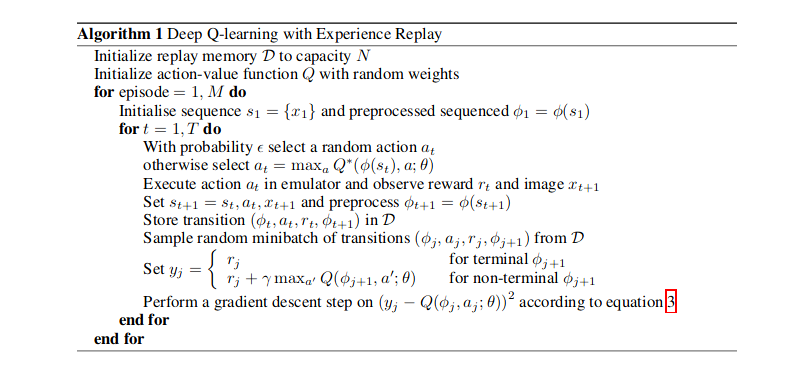
\includegraphics[width=\linewidth]{dqnalgo.png}
			\caption{DQN algortihm presentato nell'articolo \cite{nature_dqn}}
			\label{fig:dqn_algo}
		\end{figure}

	\subsection{Double Q-learning}
		Nell'articolo \textit{Deep Reinforcement Learning with Double Q-learning} di Silver et al. viene introdotta una variante dell'algoritmo DQN per attaccare il problema di sovrastimazione della funzione Q. L'algoritmo propone di disaccoppiare la selta greedy dell'azione dalla valutazione dell'azione stessa. Alla rete principale viene affiancata una seconda rete neuronale detta \textit{target network} i cui pesi $\theta^{-}$ vengono aggiornati in base ai pesi $\theta$ della rete online in maniera asincrona ogni $\tau$ passi.

		La funzione di target per il calcolo della loss diventa:\\

		$y_{i}^{D D Q N}=r+\gamma Q\left(s^{\prime}, \arg \max _{a^{\prime}} Q\left(s^{\prime}, a^{\prime} ; \theta_{i}\right) ; \theta^{-}\right)$

	\subsection{Dueling DDQN}
		Wang et al. in \textit{Dueling Network Architectures for Deep Reinforcement Learning} \cite{1511.06581} propongono una variante al modello convoluzionale usato fino a quel momento. L'intuizione su cui si basa il lavoro è che se l'agente si trova in uno stato svantaggioso non avrà importanza quale azione sceglierà. Questa idea viene concretizzata disaccoppiando l'apprendimento delle coppie $Q\left(s, a\right)$ nell'apprendimento di due funzioni separate: una che valuta il valore dello stato in cui si trova l'agente e la seconda che valuta i vantaggi derivanti dalle azioni.

		Nell'immagine \ref{fig:dueling_arch} viene visualizzata la nuova architettura che divide esplicitamente il calcolo del valore dello stato da quello delle azioni.

		\begin{figure}[H]
			\centering
			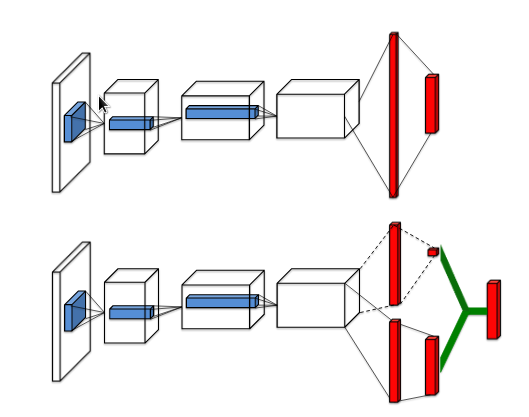
\includegraphics[width=0.5\linewidth]{dueling_arch.png}
			\caption{Immagine presa dall'articolo \cite{1511.06581}. Viene mostrata la differenza tra l'archittettura classica (in alto) con diversi strati convoluzionali e uno strato fully connected e l'archittetura proposta (in basso) che sdoppia l'ultimo strato in due flussi: il primo risulta in uno scalare e rappresenta il valore (\textit{value}) dello stato e il secondo risulta nei vantaggi (advantage) per ogni azione}
			\label{fig:dueling_arch}
		\end{figure}

	\section{Ambiente OpenAI Gym}
		Come ambiente virtuale di benchmark è stata utilizzata la Gym di OpenAI \cite{open.ai}, in particolare è stato scelto il task CartPole-v1 nel quale l'agente controlla con azioni discrete (spinta a sx, spinta a dx, nessuna azione) un carrello con un'asta attaccata ad esso da un perno (come mostrato in figura \ref{fig:cartpole}). L'obiettivo dell'agente è mantenere in equilibrio l'asta per più tempo possibile.

		\begin{figure}[H]
			\centering
			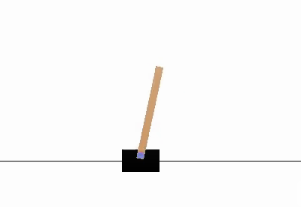
\includegraphics[width=0.3\linewidth]{cartpole.png}
			\caption{Fermo immagine di una sessione per il task CartPole-v1 di OpenAI Gym}
			\label{fig:cartpole}
		\end{figure}

		L'ambiente restituisce un reward di +1 all'agente ad ogni timestep e chiude l'episodio se l'asta supera un'inclinazione di 15 gradi o se il carrello si sposta troppo dal centro.

	\section{Implementazione}
	\subsection{Architettura del modello}
		L'architettura usata per il progetto è simile alla rete illustrata nell'immagine \ref{fig:dueling_arch} ma con una rete a 3 strati \textit{fully connected} al posto di quella convoluzionale. \\

		\begin{center}
		\begin{tabular}{| c | c |}
			\hline
			\multicolumn{2}{|c|}{rete fully connected} \\
			\hline
			\multicolumn{2}{|c|}{\textit{input} x 256} \\
			\multicolumn{2}{|c|}{256 x 128} \\
			\multicolumn{2}{|c|}{128 x 64} \\
			\hline
			value & advantage \\
			\hline
			64 x 32 & 64 x 32 \\
			32 x 1 & 32 x \textit{actions} \\
			\hline
		\end{tabular}
		\end{center}

	\subsection{Algoritmo}
		L'algoritmo si divide in una fase di inizializzazione e una fase di training. \\
		Nella fase di inizializzazione:
		\begin{itemize}
		\item viene istanziato il replay buffer e la memoria viene inizializzata in base al parametro \texttt{REPLAY\_BUFFER\_SIZE}
		\item viene istanziato il modello e vengono caricati i pesi da file se specificato. $\theta$ = $load\_or\_init()$
		\item viene creata la target network duplicando la rete appena istanziata. i pesi della rete primaria vengono copiati nella target network. $\theta^{-}$ = $\theta$
		\item viene inizializzata la variabile $\epsilon$ a \texttt{E\_START}
		\end{itemize}

		Il ciclo di training procede nel seguente modo:

		\begin{pseudocode}{Dueling DDQN}{epochs}
			\REPEAT
				s \GETS env.GetState() \\
				\REPEAT
					\IF random() <\ $\epsilon$
					$\THEN a \GETS RandomAction()$
					$\ELSE a \GETS \arg \max(Q(s; \theta))$ \\

					$s^{\prime}, r \GETS env.act(a)$ \\
					$insert (s, a, s^{\prime}, r)\ into\ ReplayBuffer$ \\

					$s_{b}, a_{b}, s_{b}^{\prime}, r_{b} \GETS ReplayBuffer.sample(BATCH\_SIZE)$ \\
					$targetY \GETS r_{b} + \gamma Q\left(s_{b}^{\prime}, \arg \max _{a_{b}^{\prime}} Q\left(s_{b}^{\prime}, a_{b}^{\prime} ; \theta\right) ; \theta^{-}\right)$ \\
					$loss \GETS MeanSquaredError(targetY - Y_{b})$ \\
					$ApplyGradients(loss, \theta)$ \\

					$every \tau\ steps\ \theta^{-} \GETS \theta$ \\
					$update\ \epsilon$

				\UNTIL $episode\_over$
			\UNTIL epochs
		\end{pseudocode}

	\subsection{Tecnologie utilizzate e dettagli implementativi}
		Tutto il progetto è stato sviluppato in python 3.7. \\
		Per l'implementazione del modello è stato utilizzato tensorflow 2.0 per l'auto differenziazione del gradiente e keras per la definizione e il training della rete neuronale. \\
		I dettagli implementativi più interessanti sono il \textit{submoduling} del modello keras per l'inserimento in maniera trasparente dell'ultimo livello che combina i flussi di value e advantage, e l'uso del \textit{gradient tape} per l'auto differenziazione di quest'ultimo. \\

		Per questo progetto ho deciso di utilizzare una variante del classico decadimento $\epsilon$-greddy dell'esplorazione resettando $\epsilon$ di nuovo al valore massimo ogni $\upsilon$ passi (per $\upsilon$ è stato usato un valore di 50000). Inoltre, il decadimento è di tipo esponenziale come si può vedere dalla figura \ref{fig:epsilon}. Questa variante dell'esplorazione $\epsilon$-greedy permette all'agente di alternare fasi di micro ottimizzazione a fasi di macro esplorazione. In particolare è stato osservato che anche con un solo reset del ciclo di esplorazione è stato possibile rompere un'abitudine "lazy" dell'agente per migliorare sensibilmente la sua performance; nel caso appena accennato l'agente aveva imparato ad "accontentarsi" di uno stato suboptimale che gli permetteva di raggiungere punteggi molto alti arrivando al limite della sua zona legale poco prima della fine degli episodi. Un reset di $\epsilon$ e poche epoche di training sono bastate a raggiungere un livello molto più alto.

		\begin{figure}[H]
			\centering
			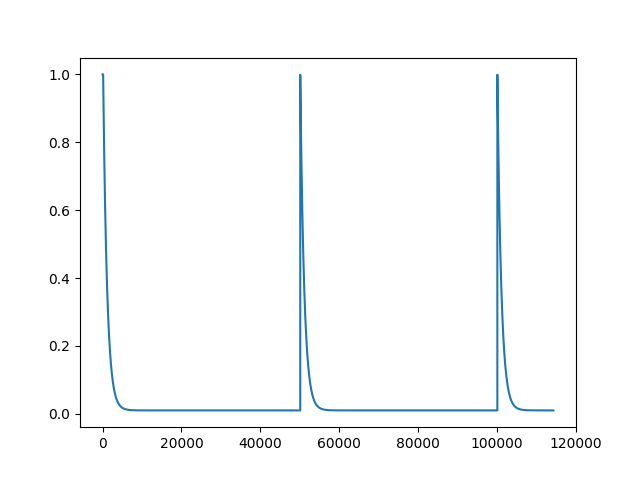
\includegraphics[width=0.8\linewidth]{epsilon.png}
			\caption{Decadimento esponenziale di $\epsilon$ con reset del ciclo}
			\label{fig:epsilon}
		\end{figure}

	\section{Risultati}
	\subsection{Parametri utilizzati}
		Durante i test sono stati utilizzati i seguenti parametri \\

		\begin{center}
		\begin{tabular}{l | r}
			Batch size & 50 \\
			Future discount $\gamma$ & 0.99 \\
			Replay buffer size & 2000 \\
			$\epsilon$ start & 1 \\
			$\epsilon$ minimum & 0.01 \\
			$\epsilon$ decay & 1000 \\
			$\epsilon$ reset frequency & 50000 \\
			Azioni per episodio & 1000 \\
		\end{tabular}
		\end{center}

	\subsection{Training e reward totali}
		In figura \ref{fig:rewards} è possibile notare il rapido incremento del punteggio ottenuto dall'agente durante le prime fasi. Successivamente è possibile notare i picchi negativi successivi al reset dei cicli di $\epsilon$-esplorazione. Sul sito del progetto \cite{git} è possibile trovare dei video dell'agente addestrato alle prove con il task sotto la cartella \textit{docs}.

		\begin{figure}[H]
			\centering
			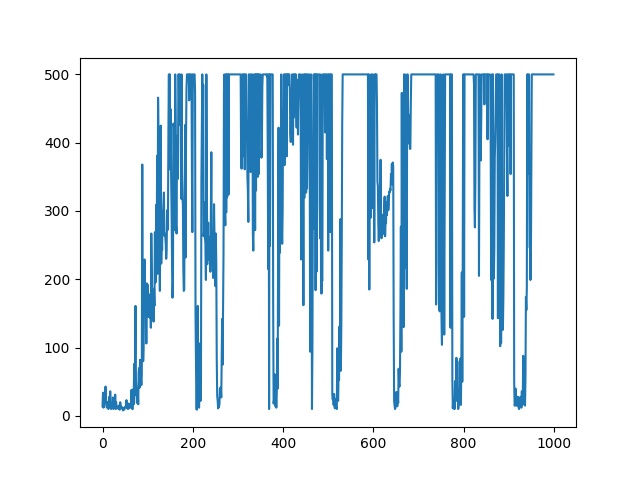
\includegraphics[width=0.8\linewidth]{rewards.png}
			\caption{Andamento del reward totale guadagnato dall'agente in fase di training}
			\label{fig:rewards}
		\end{figure}

	\newpage
	\bibliography{mybib}{}
	\bibliographystyle{plain}
\end{document}